\chapter{Theoretische Grundlagen}


\section{Sensoren}

    \subsection{Magnetometer}

    \subsection{Gyroskyp}

    \subsection{Laserscanner}

    \subsection{Kamera}

        \subsubsection{Bild Kamera}

        \subsubsection{Infrarot Kamera}

    \subsection{Abstandssensoren}

\section{ROS}

    \subsection{Nodes}

    \subsection{Topics}

    \subsection{Publish and Subscripe Pattern}

    \subsection{Objekterkennung}

    \subsection{QR-Codes}

\section{Drohne/Multicopter}
Bei der für das Projekt verwendete Drohne handelt es sich um eine Coex Clover Drohne. Dies ist eine programmierbare Drohne, die besonders für Bildungszwecke eingesetzt wird. Sie ist sowohl für den Einsatz draußen sowie auch in Gebäuden geeignet. \\

\begin{figure}[htpb]
    \centering
    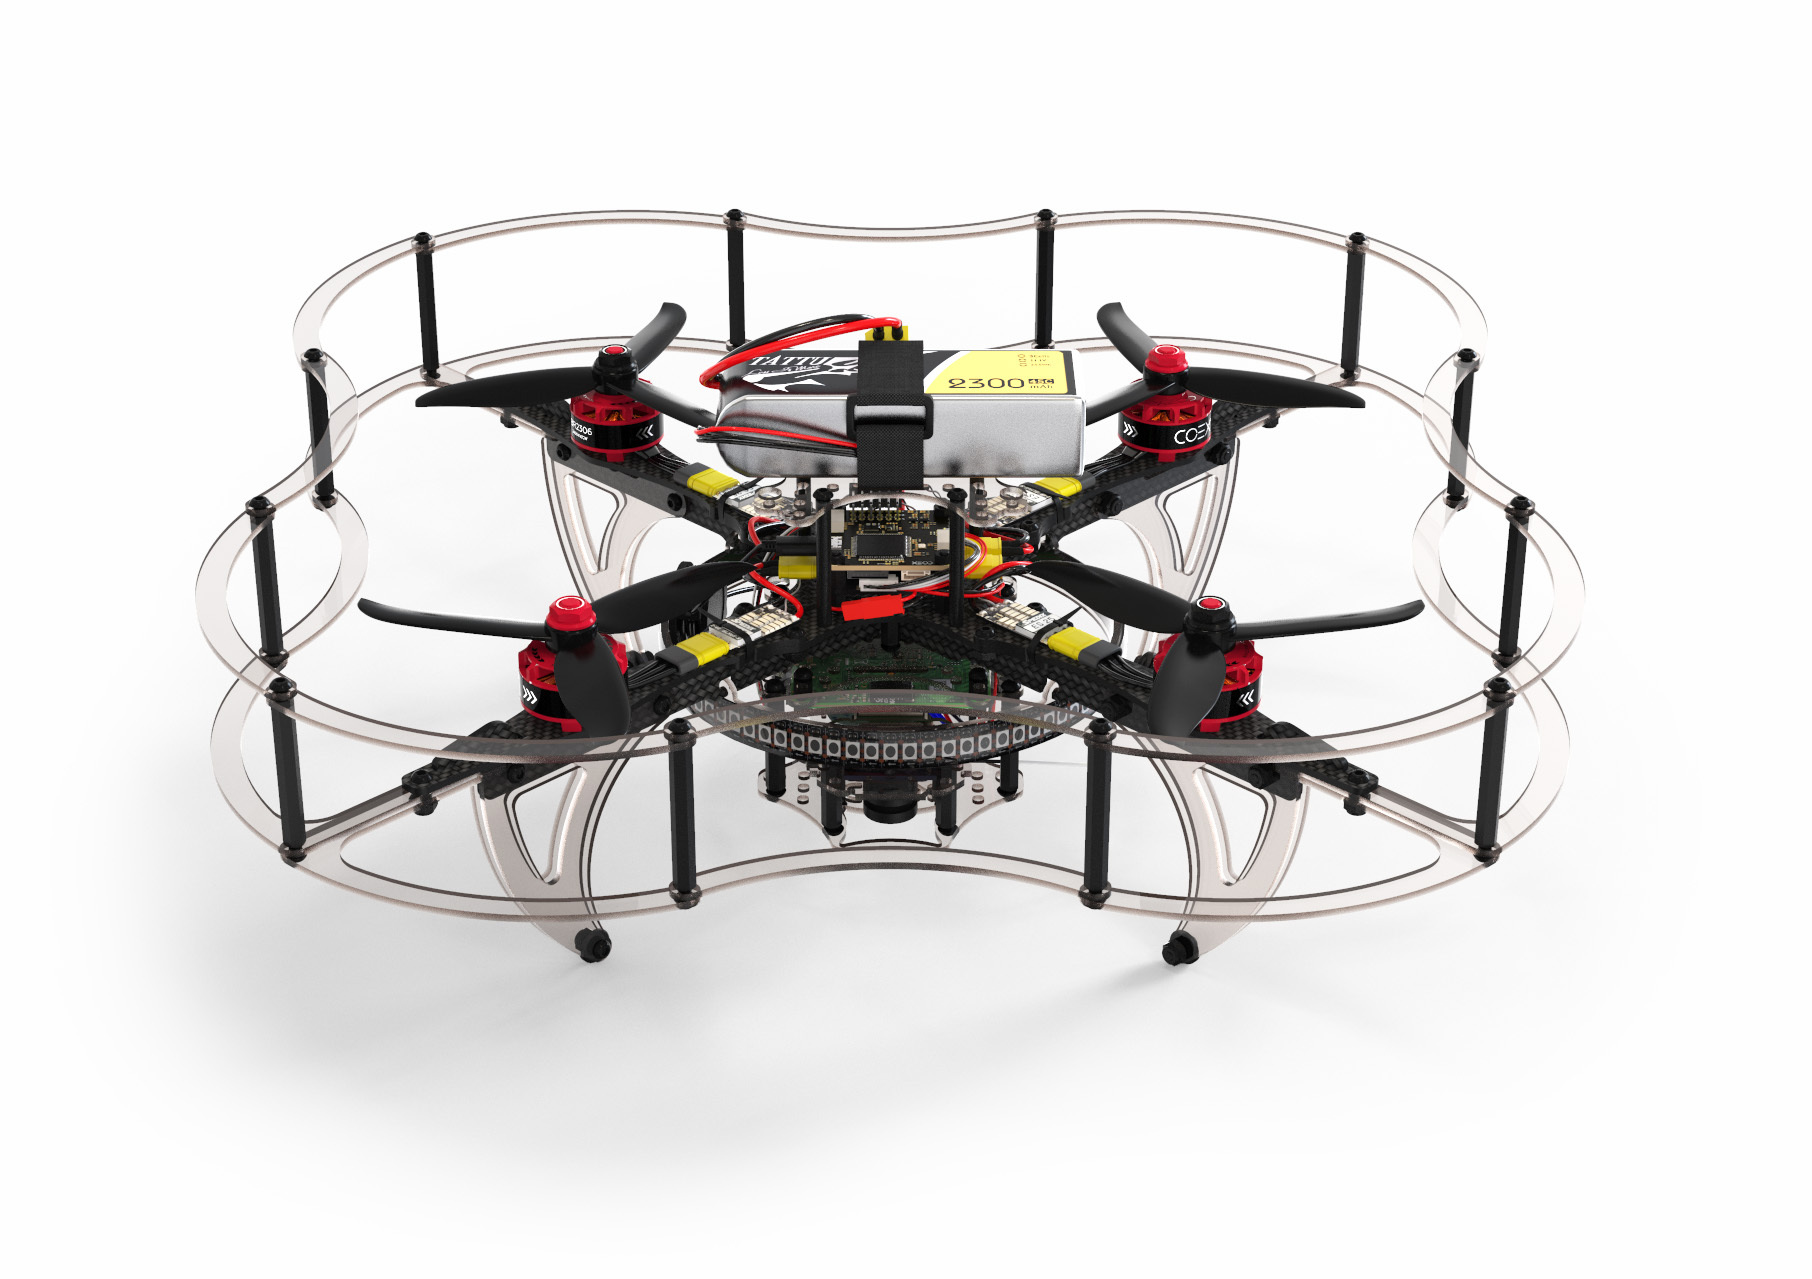
\includegraphics[width=10cm,keepaspectratio,angle=0]{images/coex_clover.jpg}
    \caption[Coex Clover Drohne]{\label{img coex_clover} Coex Clover Drohne \cite{img_coex_clover}}
\end{figure}

Zu Beginn erhält man hierbei einen Bausatz, welcher dann zu einem Quadrokopter zusammengebaut werden kann. Der Vorteil hierbei ist zudem, dass die gesamte Drohne ohne Löten zusammengesetzt werden kann. Zu den einzelnen Bestandteilen der Drohne kommen, noch eine Dokumentation sowie verschiedene Bibliotheken, die es ermöglichen, die Drohne zusammen bauen und fliegen lassen zu können. \\
Die 
Durch die Verwendung verschiedener Open-Source Komponenten lässt sich die Drohne programmieren, wodurch ein vielseitiger Einsatzbereich entsteht.\\

\begin{figure}[htpb]
    \centering
    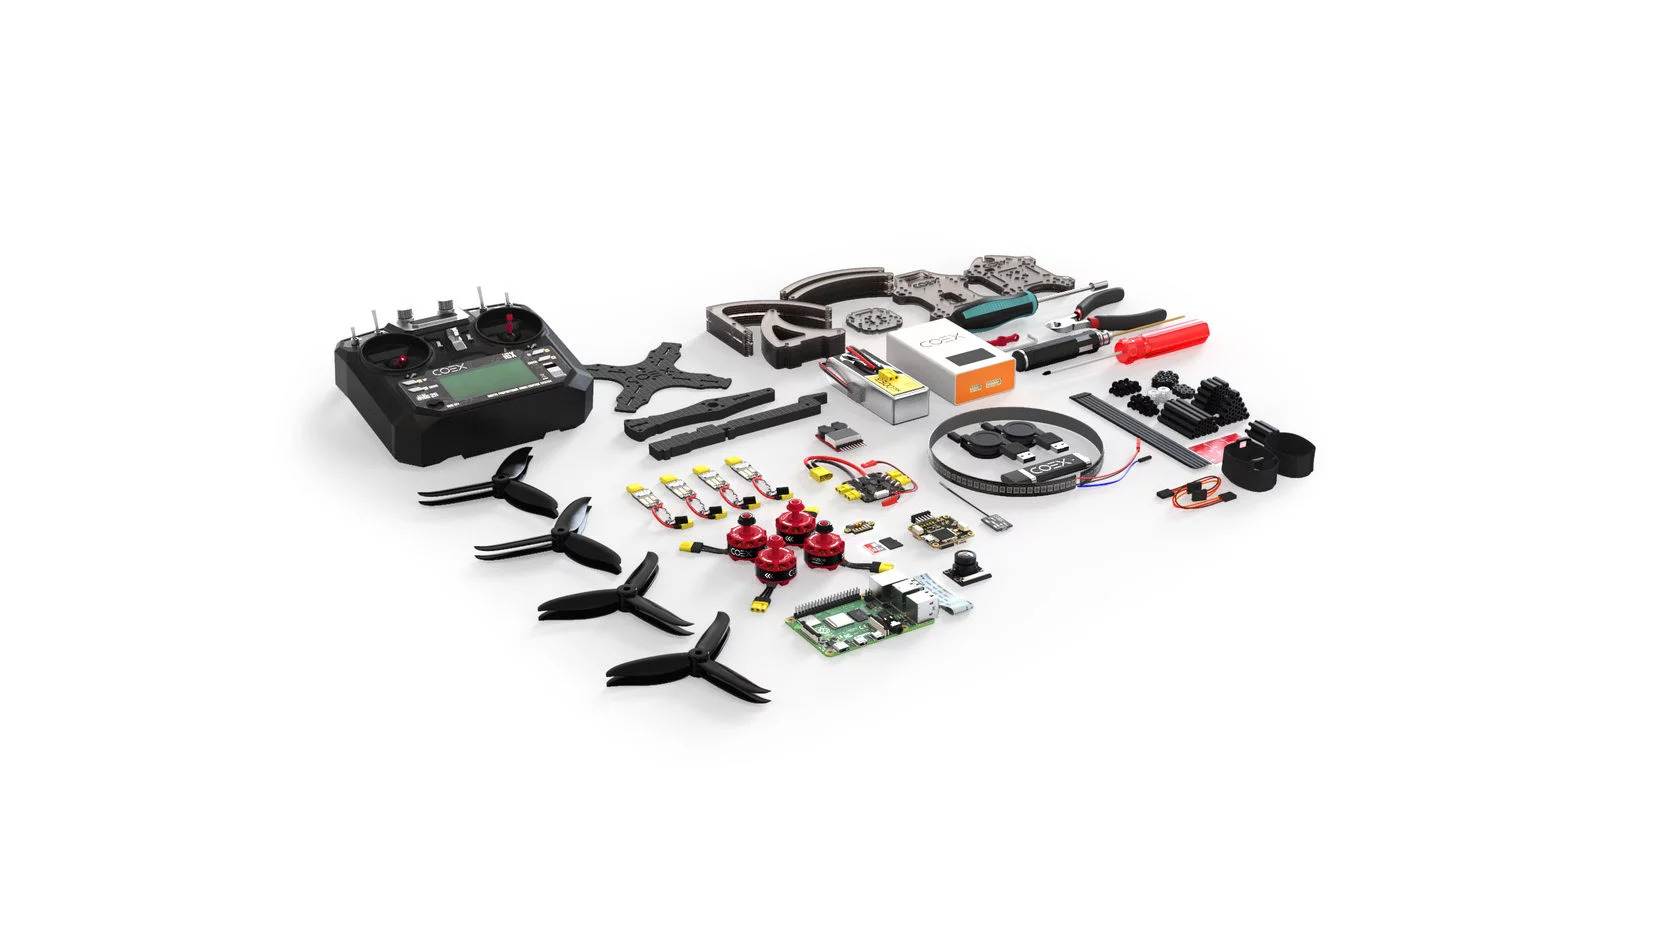
\includegraphics[width=10cm,keepaspectratio,angle=0]{images/coex_clover_kit.jpg}
    \caption[Bausatz Coex Clover Drohne]{\label{img coex_clover_kit} Bausatz Coex Clover Drohne \cite{img_coex_clover_kit}}
\end{figure}

Die Coex Clover Drohne soll laut Herstellerinformationen bis zu 15 Minuten am Stück fliegen können und in dieser Zeit eine Maximalhöhe von 500 Metern bei einer Höchstgeschwindigkeit von bis zu 72 km/h erreichen können \cite[vgl.][]{coex_clover}.\\

Es gibt verschiedene Versionen der Drohne, bei der hier eingesetzten, handelt es sich um die Coex Clover 4.2.
Wichtige Bestandteile dieser sind hierbei:
\begin{center}
    \begin{itemize}
        \item Flight-Controller Coex Pix
        \item Raspberry Pi 4
        \item 
        \item 
        \item 
        \item 
    \end{itemize}
    \label{lst:coex-components}
\end{center}

Zu den Hauptbestandteilen der Drohne zählen zum einen ein Raspberry Pi 4 sowie der Flightcontroller Coex Pix. Diese bilden die Grundlage zur Programmierung und Steuerung der Coes Clover Drohne und ermöglichen es zudem die Drohne über drahtlos per WLAN zu verbinden. \\
Die Drohne ist ein Quadrokopter und besitzt somit vier Motoren, welche einzelnd angesteuert werden können. Sie besitzt zudem eine Vielzahl verschiedener Sensoren, auf welche in \ref{section:Sensoren} genauer eingegangen wird. Zu diesen zählen unter anderem ein Gyroskop, Magnetometer sowie ein Laseranstandssensor und eine Kamera, die unten an der Drohne angebracht sind.
Zum Schutz befindet sich zudem außen einen Rahmen.



\section{3D-Modelle}

    \subsection{3D-Scanning}

\section{Positionsbestimmung}

    \subsection{Spatial Mapping}

    \subsection{Inertielle Positionsbestimmung}

\section{Regelsysteme}

    \subsection{PID-Regler}

\section{Simulationstechnik}

\section{Problembehebung}
